\section{Laboratory work implementation}

\subsection{Tasks and Points}

\begin{enumerate}
\item Realizeaza un simplu GUI calculator care suporta urmatoare functii: +, -, /, *, putere, radical, InversareSemn(+/-), operatii cu numere zecimale.
\item Divizare proiectului in doua module - Interfata grafica(Modul GUI) si Modulul de baza(Core Module).
\end{enumerate}

\subsection{Analiza lucrarii de laborator}

\begin{enumerate}
\item Primul pas a fost inițializarea unui nou repozitoriu pe GitHub și clonarea acestuia pe calculatorul personal: \url{https://github.com/emirovschi/MIDPS\-2}.
\item Proiectul a fost creat utilizând IntelliJ\cite{IntelliJ} și folosind Maven\cite{Maven} ca build manager. Acesta oferă posibilitatea de a adăuga automat toate dependențele inclusiv cele tranzitive.
\item Acest proiect este compus din 2 module:
\begin{enumerate}
\item [\textbf{core}] Conține toată logica de calcul și conversie a numerelor din șir de caractere în numere cu virgula mobilă;
\item [\textbf{gui}] Este dependent de GUI framework și conține descrierea interfeței grafice precum și setul de acțiuni care vor fi executate pentru diferite tipuri de evenimente gen apăsare de buton virtual sau fizic.
\end{enumerate}
Maven ofera posibilitatea de a defini aceste module care la rândul său vor deveni proiecte de acest tip și vor avea fișierul propriu cu configurare.

\begin{minipage}{\linewidth}
	\centering
	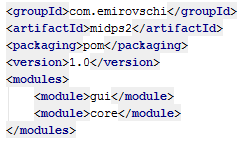
\includegraphics{modules}
	\captionof{figure}{Crearea modulelor in Maven}
\end{minipage}
\break

\item Interfața grafică a fost creată utilizând framework-ul gratuit Apache Pivot\cite{Pivot}. Componentele vizuale sunt definite utilizând un fișier XML iar legătura bidirecțională se face automat folosind anotarea \textbf{@BXML}. Acest framework permite extinderea componentelor existente pentru a adăuga careva funcționalități noi sau comportament specific.

\begin{minipage}{\linewidth}
	\centering
	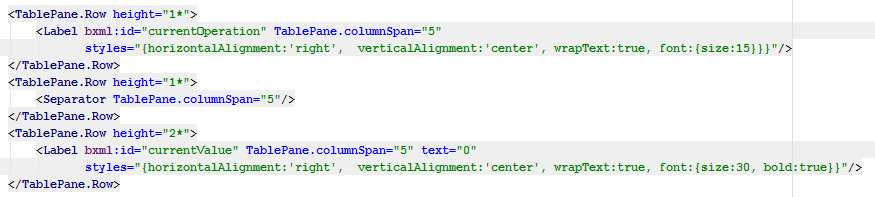
\includegraphics[width=17cm]{xml}
	\captionof{figure}{Definirea interfeței grafice folosind fișierul de configurare XML}
\end{minipage}
\break

\begin{minipage}{\linewidth}
	\centering
	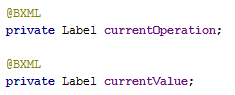
\includegraphics{bxml}
	\captionof{figure}{Crearea legăturii între componente și variabile utilizând anotația \textbf{@BXML}}
\end{minipage}
\break
\item Asocierea evenimentelor pentru butoane se face utilizând tipul componentelor. Respectiv fiecare buton va avea propriul său comportament.

\begin{minipage}{\linewidth}
	\centering
	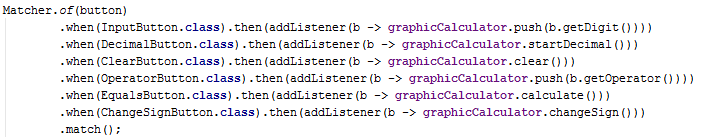
\includegraphics[width=17cm]{events}
	\captionof{figure}{Adăugarea evenimentelor}
\end{minipage}
\break
\end{enumerate}

\break
\subsection{Imagini}

\begin{figure}[ht]
	\centering
	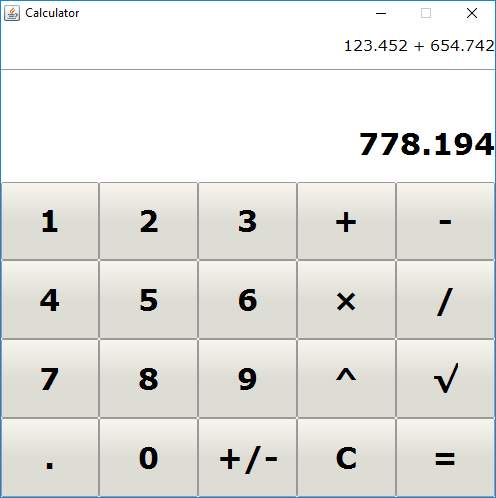
\includegraphics[width=5.5cm]{calcWrite}
	\caption{Exemplu de calcul}
\end{figure}

\begin{figure}[ht]
	\centering
	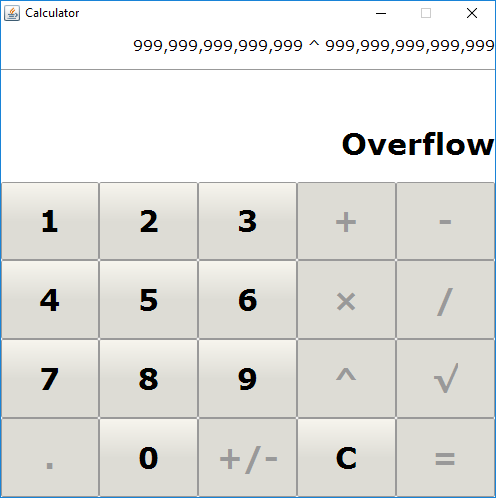
\includegraphics[width=5.5cm]{calcOverflow}
	\caption{Exemplu de exces}
\end{figure}

\begin{figure}[ht]
	\centering
	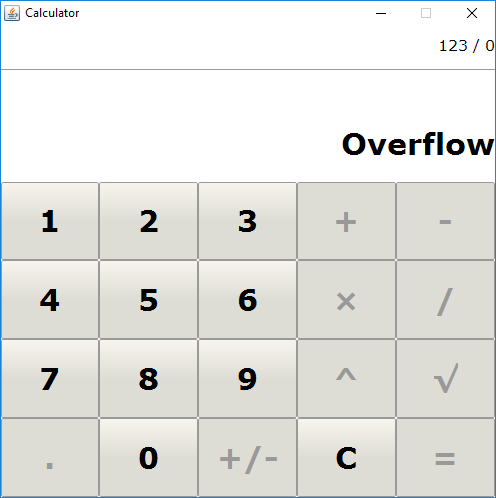
\includegraphics[width=5.5cm]{calcZero}
	\caption{Divizarea la zero}
\end{figure}

\clearpage